\chapter{文獻管理工具}
\label{chap:2}

该章节为文献管理,其目标是从下列各出版物/中找出近 5 年来与自己的研究方向相关的 100 篇文章,按照北京大学学位论文对参考文献要求,采用 Endnote、Mendeley、Zotero、Citavi、Papers 等任一种软体,规范管理文章,并将统一格式管理的结果用 LaTeX 排版展示,并对采用的管理软体做评价或体会。而文献来源如下列所示 :

\begin{itemize}

\item [-]IEEE Transaction/Magazine/Journal

\item [-]IET (IEE) Proceeding/Magazine/Journal

\item [-]ACM

\item [-]Springer

\item [-]Elsevier

\item [-]Google 学术

\item [-]Beidu 学术

\end{itemize}

而考量过可取得与开源的方案,本作业决定使用 Zotero 作为文献管理上的使用工具。

\begin{figure}[htb]
\centering 
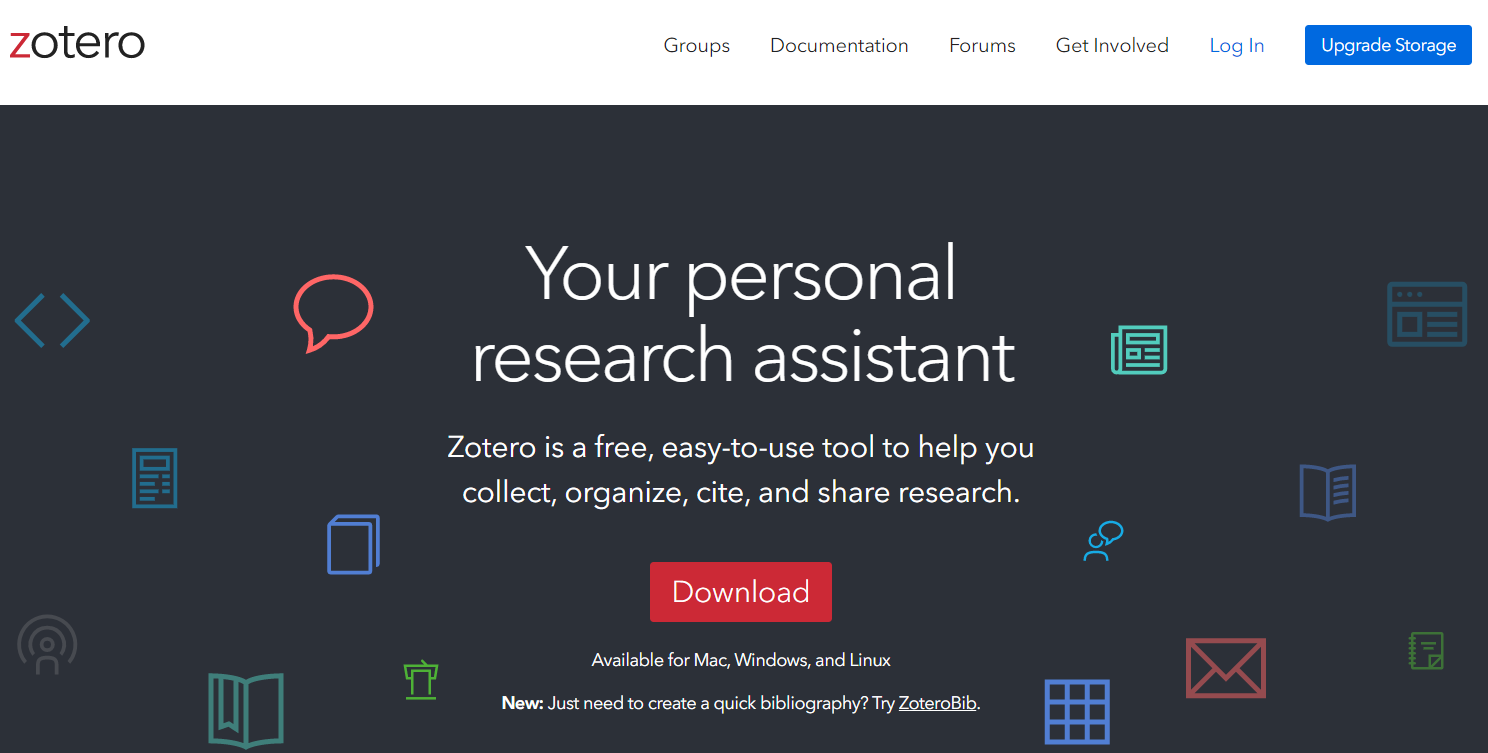
\includegraphics[width=0.90\textwidth]{img/c2m0.png} 
\caption{官网}
\label{Test}
\end{figure}

\subsection{Zotero 简介}

Zotero 是一款自由且开放原始码的文献管理软体,可支援管理文献资讯,包含如作者、标题、出版社、摘要、阅读笔记等及相关材料,比如 PDF 档案等。当中最著名的特性是作为浏览器插件状态下,可进行在线同步与文书编辑软体来产生参考文献,而文书软体包含如下 Microsoft Word、LibreOffice、OpenOffice.org Writer、NeoOffice 等集成工具,同时还可以生成文内引用与生成页面脚注或文后的参考文献(bibliographies)。

\begin{figure}[htb]
\centering 
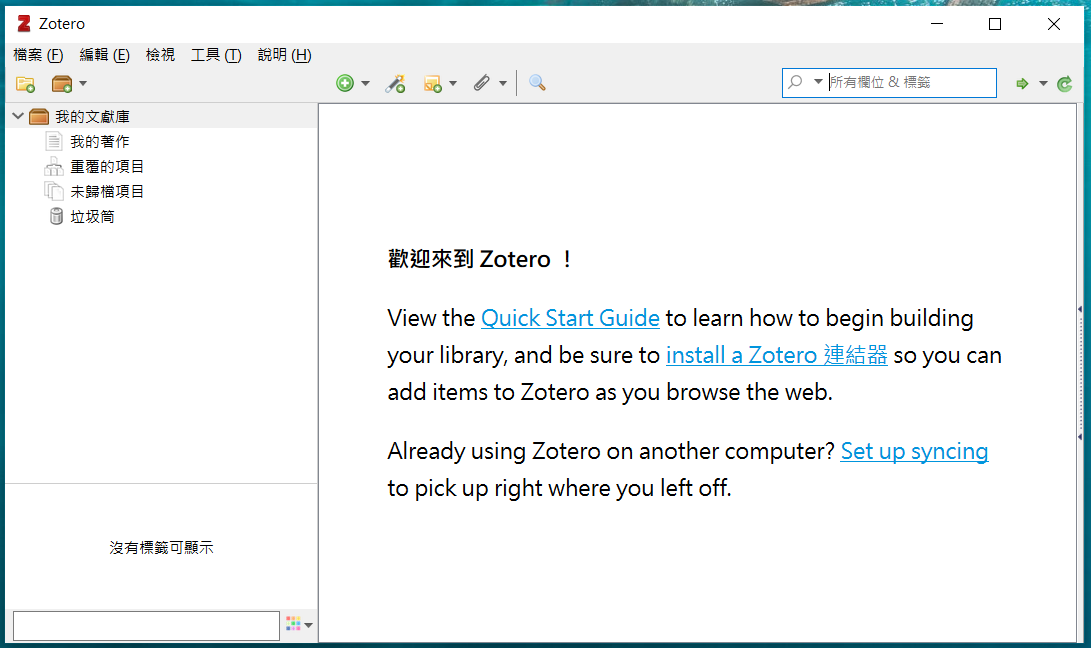
\includegraphics[width=0.90\textwidth]{img/c2m1.png} 
\caption{安装完成}
\label{Test}
\end{figure}

在此可以由官网上进行下载 (https://www.zotero.org/),并安装属于自己的版本,由于环境的作业系统是 Windows 10 ,所以选择 Windows 的版本。而安装 Zotero 完后可以看到安装完成的画面,同时也可以看到整个 Zotero 简洁的操作介面。 

\subsection{Zotero 操作}

至于浏览器的插件插入后的可以直接对文献进行纪录,在进入页面后就可以根据图形介面进行操作,方便使用者随时可以进行记录,并进行同步到文献库中,从而加速研究的工作流程。

\begin{figure}[htb]
\centering 
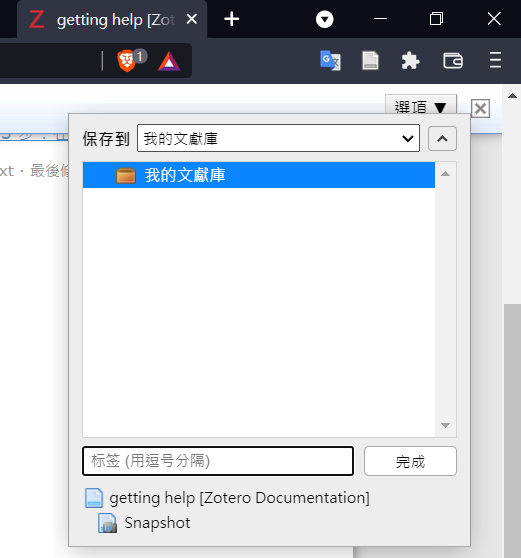
\includegraphics[width=0.50\textwidth]{img/c2m2.png} 
\caption{浏览器的插件}
\label{Test}
\end{figure}

从 Zotero 汇出 Zotero PDF 的参考文献的格式,同时可以看到 *.rdf 的格式,该格式可以汇入 Zotero 后,方便使用者进行管理。而汇出文献酷的动作,能让使用者自由选择想要用什么格式进行汇出。

\begin{figure}[htb]
\centering 
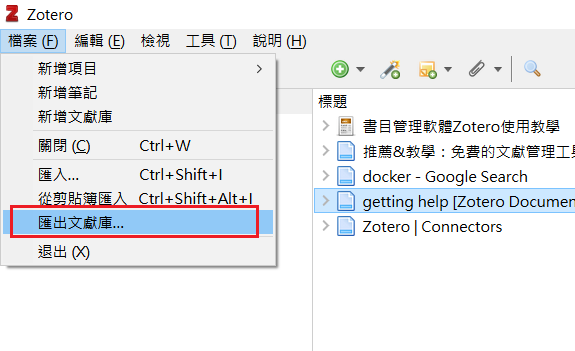
\includegraphics[width=0.50\textwidth]{img/c2m3.png} 
\caption{汇出文献库}
\label{Test}
\end{figure}

\begin{figure}[htb]
\centering 
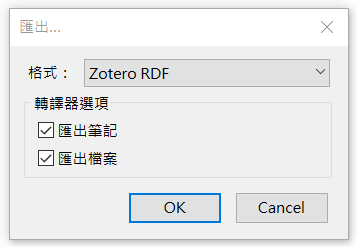
\includegraphics[width=0.50\textwidth]{img/c2m4.png} 
\caption{汇出 RDF 格式}
\label{Test}
\end{figure}

\begin{figure}[htb]
\centering 
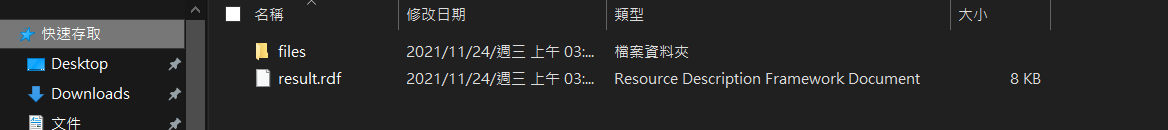
\includegraphics[width=0.95\textwidth]{img/c2m5.png} 
\caption{RDF 格式}
\label{Test}
\end{figure}

在图中可以看到汇出 CSV 格式的部分,而 CSV 格式在一些特定状况下比较好运用,在此使用 LiberOffice 来开启 CSV 格式档案,并且选择 UTF-8 格式,同时可以从 LiberOffice 中看到文献的资料。

\begin{figure}[htb]
\centering 
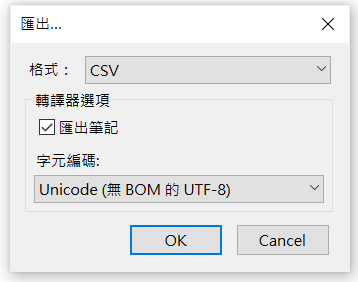
\includegraphics[width=0.40\textwidth]{img/c2m6.png} 
\caption{汇出 CSV 格式}
\label{Test}
\end{figure}

在此进行额外的说明,LiberOffice 是文书编辑软体中的一种,其开发者最早从 OpenOffice 中分离出来,该软体也与 Zotero 同为自由的开放原始码软体,同时也都支援 Mac、Windows、Linux 等多种作业系统与环境上的使用,其开放原始码授权的软体优势在于方便使用者取得跟使用且不售商业授权的影响。

\begin{figure}[htb]
\centering 
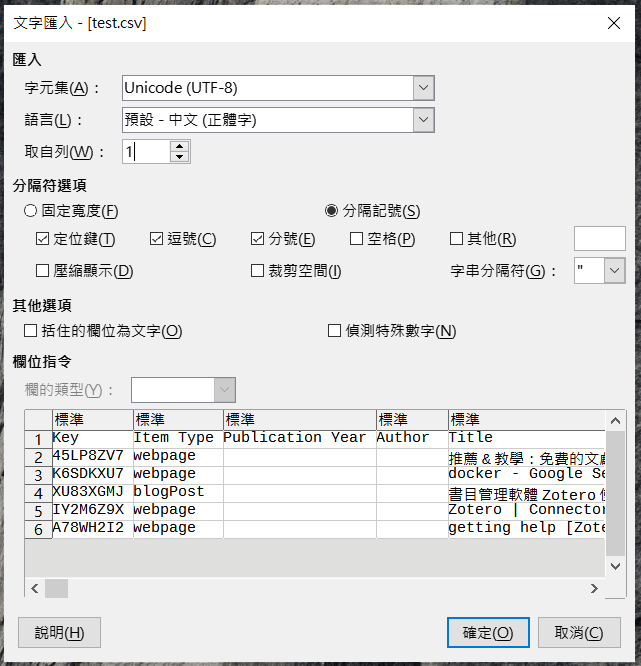
\includegraphics[width=0.90\textwidth]{img/c2m7.png} 
\caption{LiberOffice 设定}
\label{Test}
\end{figure}

\begin{figure}[htb]
\centering 
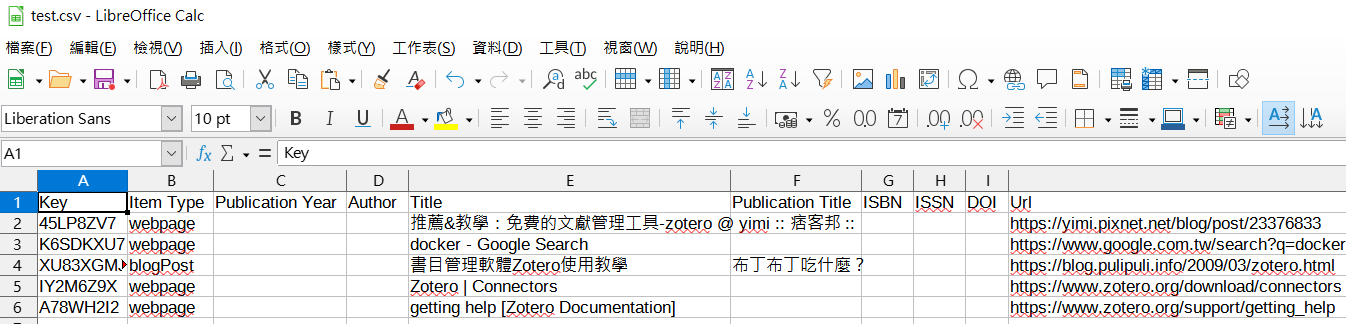
\includegraphics[width=0.95\textwidth]{img/c2m8.png} 
\caption{检视 LiberOffice 格式的文献资料}
\label{Test}
\end{figure}

最后最为重要的部分则是汇出成 LaTeX 所需要的参考文献格式,由于该课业的目标是要将参考文献汇出成北京大学硕士论文的格式,因而在此步骤非常的重要。而完成后可以看到一个 bib 格式的档案,该格式可以使用在 Overleaf 平台上,而  Overleaf 则是一个专门支援 LaTeX 文件多人协作的平台,而且拥有大量支援多校与学术科学研究的 LaTeX 模板,使用者不用花太多的心力去照顾 LaTeX 本地端环境,从而将新手的学习门槛压低。同时 Overleaf 上面已经有志愿者对北京大学博硕士论文的 LaTeX 模板进行贡献,所以后续的参考文献工作则是使用 Overleaf 的北京大学模板,同时也是该作业的格式,该模板与平台等使用详细资讯则由下一章进行详述。

\begin{figure}[htb]
\centering 
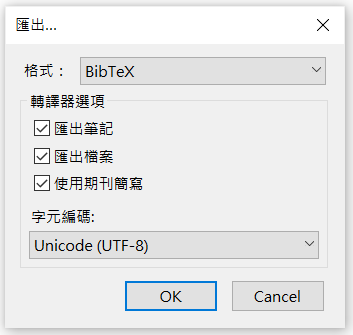
\includegraphics[width=0.40\textwidth]{img/c2m9.png} 
\caption{BibTeX}
\label{Test}
\end{figure}

\begin{figure}[htb]
\centering 
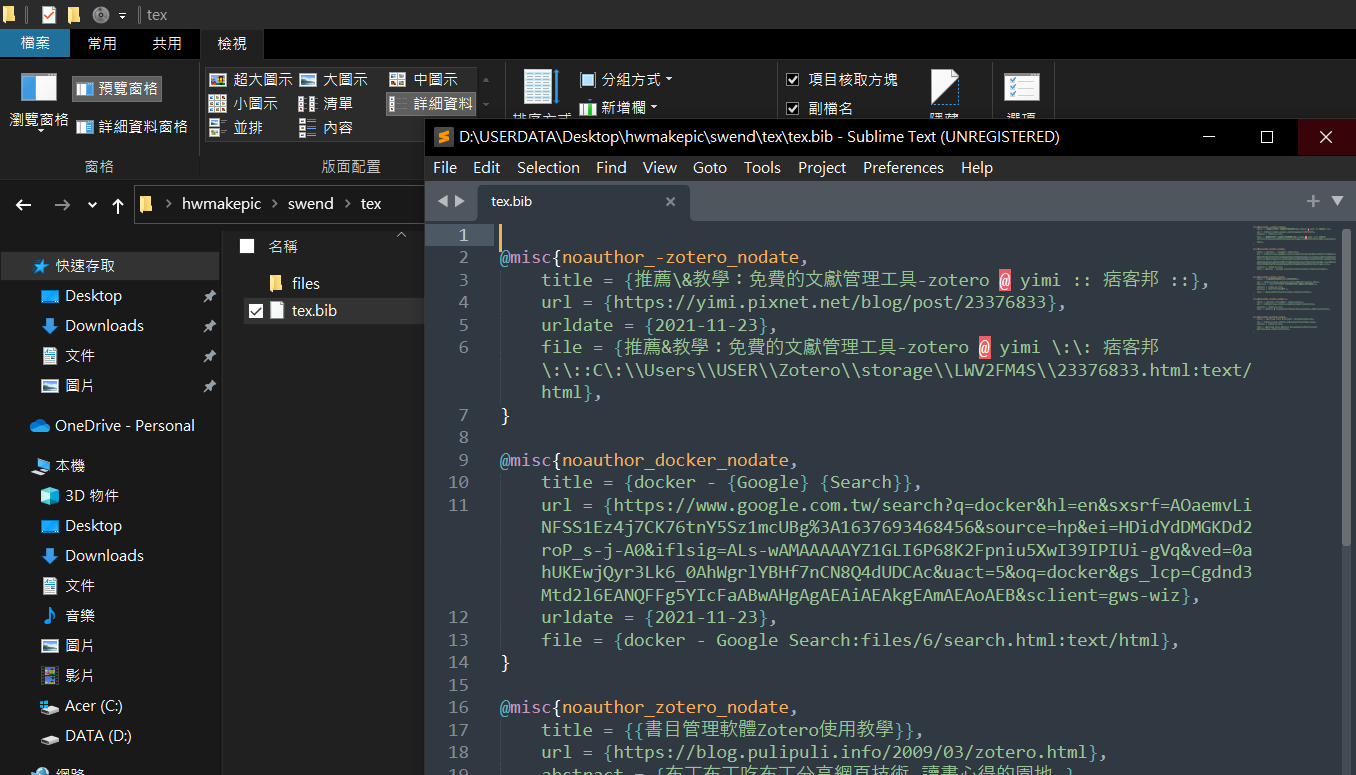
\includegraphics[width=0.90\textwidth]{img/c2m10.png} 
\caption{LaTeX 的 bib 格式}
\label{Test}
\end{figure}

